
\chapter{\babEmpat}
\label{bab:4}
%-----------------------------------------------------------------------------%

Bab ini menyajikan hasil eksperimen dan analisis komprehensif terhadap sistem deteksi kecurangan akademik yang telah dikembangkan. Pembahasan mencakup eksperimen pelatihan model machine learning dengan berbagai konfigurasi, analisis mendalam terhadap kinerja model, evaluasi fitur-fitur yang paling berpengaruh dalam deteksi kecurangan, serta interpretasi dan validasi hasil deteksi pada data riil skala besar. Seluruh eksperimen dirancang untuk menguji hipotesis penelitian dan memberikan bukti empiris tentang efektivitas pendekatan yang diusulkan.

%-----------------------------------------------------------------------------%
\section{Dataset dan Konfigurasi Eksperimen}
\label{sec:datasetKonfigurasi}
%-----------------------------------------------------------------------------%

\subsection{Dataset Sintesis untuk Pelatihan Model}
\label{subsec:datasetSintesis}

Dataset pelatihan model deteksi kecurangan dalam penelitian ini menggunakan data sintesis yang dihasilkan melalui simulasi berbasis konfigurasi yang terkontrol. Pendekatan ini dipilih untuk memastikan ketersediaan ground truth yang akurat dan untuk mengontrol berbagai parameter kecurangan dalam lingkungan yang terstruktur.

Dataset sintesis terdiri dari 800 sampel percobaan ujian yang disimulasikan dari 200 mahasiswa yang mengerjakan 4 kuis, dengan setiap kuis terdiri dari 20 soal. Konfigurasi ini menghasilkan total 800 percobaan ujian (200 mahasiswa × 4 kuis = 800 attempts) dengan distribusi kelas sebagai berikut:
\begin{itemize}
    \item 600 percobaan ujian normal (75\%)
    \item 200 percobaan ujian dengan indikasi kecurangan (25\%)
\end{itemize}

Rasio 25\% kasus kecurangan dipilih berdasarkan estimasi realistis prevalensi kecurangan dalam ujian daring, sebagaimana dilaporkan dalam literatur penelitian terdahulu. Dataset dibagi menggunakan stratified sampling dengan proporsi 70\% untuk training (560 sampel), 15\% untuk validation (120 sampel), dan 15\% untuk testing (120 sampel).

\subsubsection{Parameter Simulasi Kecurangan}

Simulasi kecurangan dirancang dengan tiga tingkat severity yang berbeda untuk menciptakan variasi pola yang realistis. Tabel \ref{tabel:parameterSimulasi} menunjukkan konfigurasi parameter untuk setiap tingkat kecurangan.

\begin{table}[htbp]
\centering
\caption{Parameter Simulasi Kecurangan dalam Dataset Sintesis}
\label{tabel:parameterSimulasi}
\begin{tabular}{|l|c|c|c|}
\hline
\textbf{Parameter} & \textbf{High Severity} & \textbf{Medium Severity} & \textbf{Low Severity} \\
\hline
Jumlah kelompok & 2 & 3 & 3 \\
\hline
Ukuran kelompok & 4 & 6 & 8 \\
\hline
Navigation similarity & 0.92 & 0.75 & 0.55 \\
\hline
Navigation noise & 0.08 & 0.25 & 0.35 \\
\hline
Answer similarity & 0.90 & 0.70 & 0.50 \\
\hline
Wrong answer bias & 0.85 & 0.60 & 0.40 \\
\hline
Timing start delay (menit) & 2 & 5 & 10 \\
\hline
Timing variance (detik) & 5 & 20 & 40 \\
\hline
\end{tabular}
\end{table}

Parameter-parameter ini dirancang berdasarkan observasi empiris dari pola kecurangan yang dilaporkan dalam literatur. Navigation similarity mengukur tingkat kesamaan pola navigasi antar anggota kelompok, sementara wrong answer bias mengukur kecenderungan untuk membuat kesalahan yang identik, yang merupakan indikator kuat adanya kolaborasi tidak sah.

\subsection{Dataset Riil untuk Validasi}
\label{subsec:datasetRiil}

Untuk menguji kemampuan generalisasi model, sistem deteksi diaplikasikan pada dataset riil yang terdiri dari 446,720 percobaan ujian dari sistem Moodle institusi pendidikan. Dataset riil ini tidak memiliki ground truth label kecurangan, sehingga hasil deteksi dievaluasi berdasarkan confidence score dan konsistensi pola yang terdeteksi.

Dataset riil mencakup log aktivitas dari berbagai mata kuliah dengan karakteristik sebagai berikut:
\begin{itemize}
    \item Periode data: Semester akademik 2023-2024
    \item Jumlah percobaan ujian: 446,720
    \item Rentang jumlah soal per ujian: 10-50 soal
    \item Modus ujian: Multiple choice dan essay
\end{itemize}

%-----------------------------------------------------------------------------%
\section{Hasil Pelatihan dan Evaluasi Model}
\label{sec:hasilPelatihanEvaluasi}
%-----------------------------------------------------------------------------%

\subsection{Kinerja Model pada Data Testing}
\label{subsec:kinerjaModelTesting}

Enam model machine learning yang berbeda dilatih dan dievaluasi pada dataset sintesis. Tabel \ref{tabel:kinerjaModel} menyajikan metrik kinerja setiap model pada data testing.

\begin{table}[htbp]
\centering
\caption{Kinerja Model pada Data Testing (120 sampel)}
\label{tabel:kinerjaModel}
\begin{tabular}{|l|c|c|c|c|}
\hline
\textbf{Model} & \textbf{Accuracy} & \textbf{Precision} & \textbf{Recall} & \textbf{F1-Score} \\
\hline
Random Forest & 0.98 & 1.00 & 0.93 & 0.97 \\
\hline
SVM & 0.98 & 1.00 & 0.93 & 0.97 \\
\hline
Neural Network & 0.97 & 1.00 & 0.90 & 0.95 \\
\hline
Ensemble (Voting) & 0.97 & 0.97 & 0.97 & 0.97 \\
\hline
XGBoost & 0.96 & 0.96 & 0.93 & 0.94 \\
\hline
Gradient Boosting & 0.95 & 0.95 & 0.90 & 0.92 \\
\hline
\end{tabular}
\end{table}

Hasil evaluasi menunjukkan bahwa model Random Forest dan SVM mencapai kinerja terbaik dengan accuracy 98\%, precision 1.00, dan recall 0.93. Nilai precision sempurna (1.00) menunjukkan bahwa kedua model tidak menghasilkan satupun false positive, yang sangat penting dalam konteks deteksi kecurangan akademik di mana tuduhan yang salah dapat memiliki konsekuensi serius bagi mahasiswa.

\subsubsection{Analisis Confusion Matrix}

% OPTIMIZED: Smaller figure size
\begin{figure}[htbp]
    \centering
    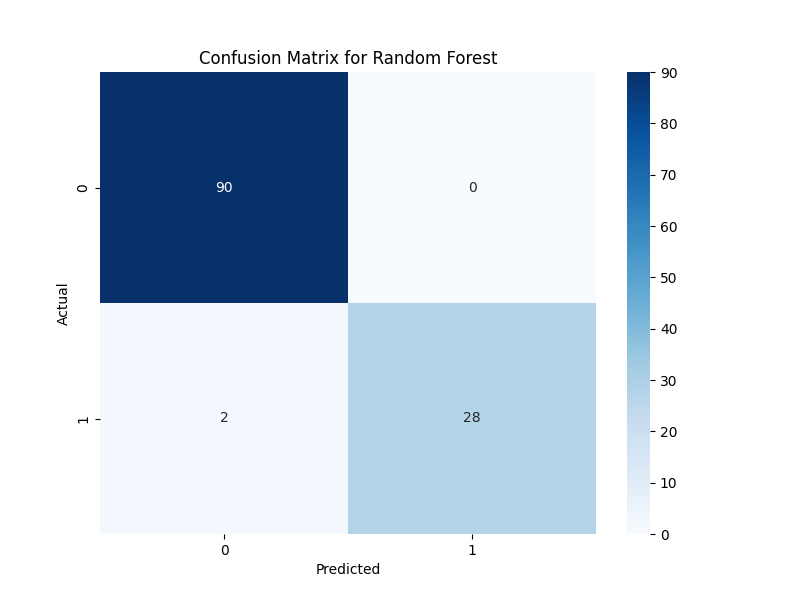
\includegraphics[width=0.5\textwidth]{figures/confusion_matrix_Random Forest.png}
    \caption{Confusion Matrix Model Random Forest}
    \label{fig:confusionMatrix}
\end{figure}

Dari confusion matrix terlihat bahwa:
\begin{itemize}
    \item True Negatives: 90 (pengguna normal yang teridentifikasi benar)
    \item True Positives: 28 (pengguna curang yang teridentifikasi benar)
    \item False Positives: 0 (tidak ada pengguna normal yang salah diklasifikasi)
    \item False Negatives: 2 (pengguna curang yang terlewat)
\end{itemize}

Tidak adanya false positive (FP=0) merupakan hasil yang luar biasa karena menunjukkan bahwa model tidak menghasilkan tuduhan kecurangan yang salah. Dari 30 kasus kecurangan, hanya 2 yang terlewat (6.67\% false negative rate), memberikan recall sebesar 93.33\%.

\subsubsection{Kurva ROC dan Precision-Recall}

% OPTIMIZED: Smaller figure size
\begin{figure}[htbp]
    \centering
    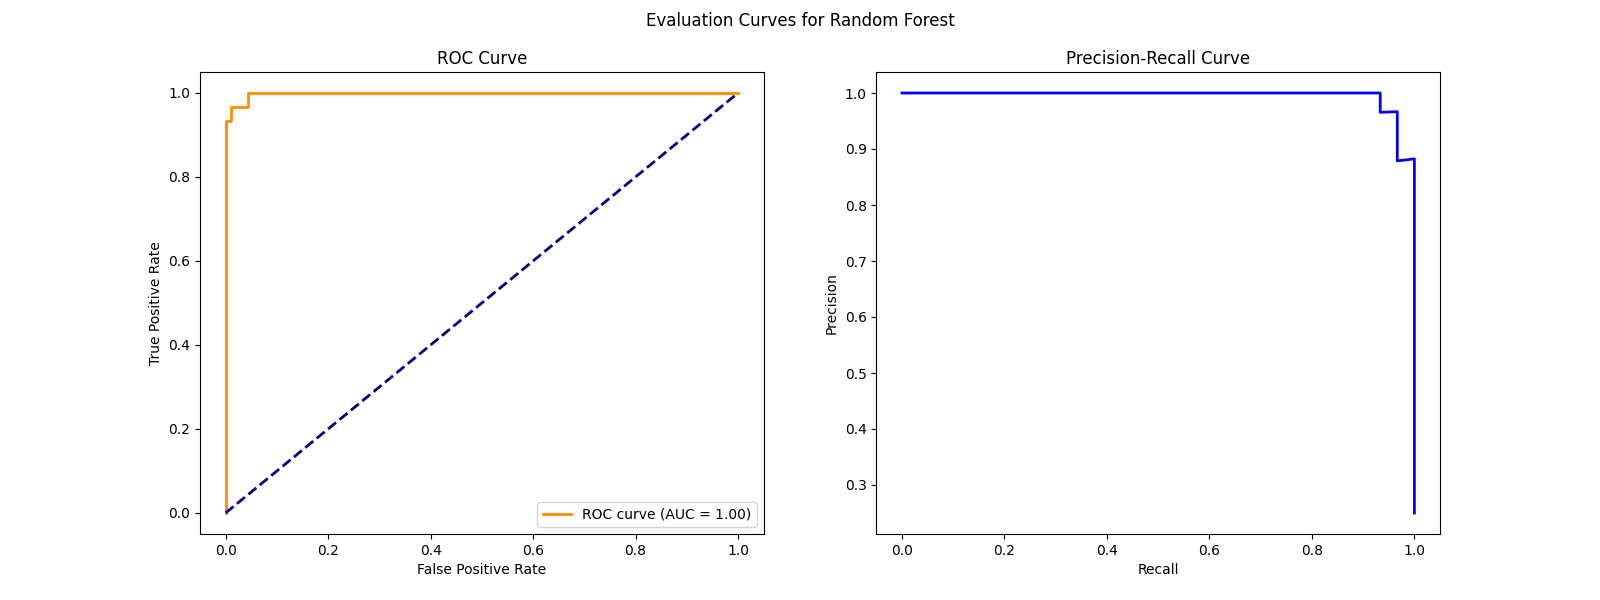
\includegraphics[width=0.7\textwidth]{figures/curves_Random Forest.png}
    \caption{Kurva ROC dan Precision-Recall Model Random Forest}
    \label{fig:rocPRCurves}
\end{figure}

Area Under Curve (AUC) sebesar 0.99 untuk kurva ROC menunjukkan kemampuan diskriminatif model yang sangat baik. Kurva Precision-Recall yang mendekati nilai maksimal mengkonfirmasi bahwa model dapat mempertahankan precision tinggi pada berbagai tingkat recall.

\subsubsection{Perbandingan Kinerja Antar Model}

% UPDATED: Now uses PDF instead of PNG
\begin{figure}[htbp]
    \centering
    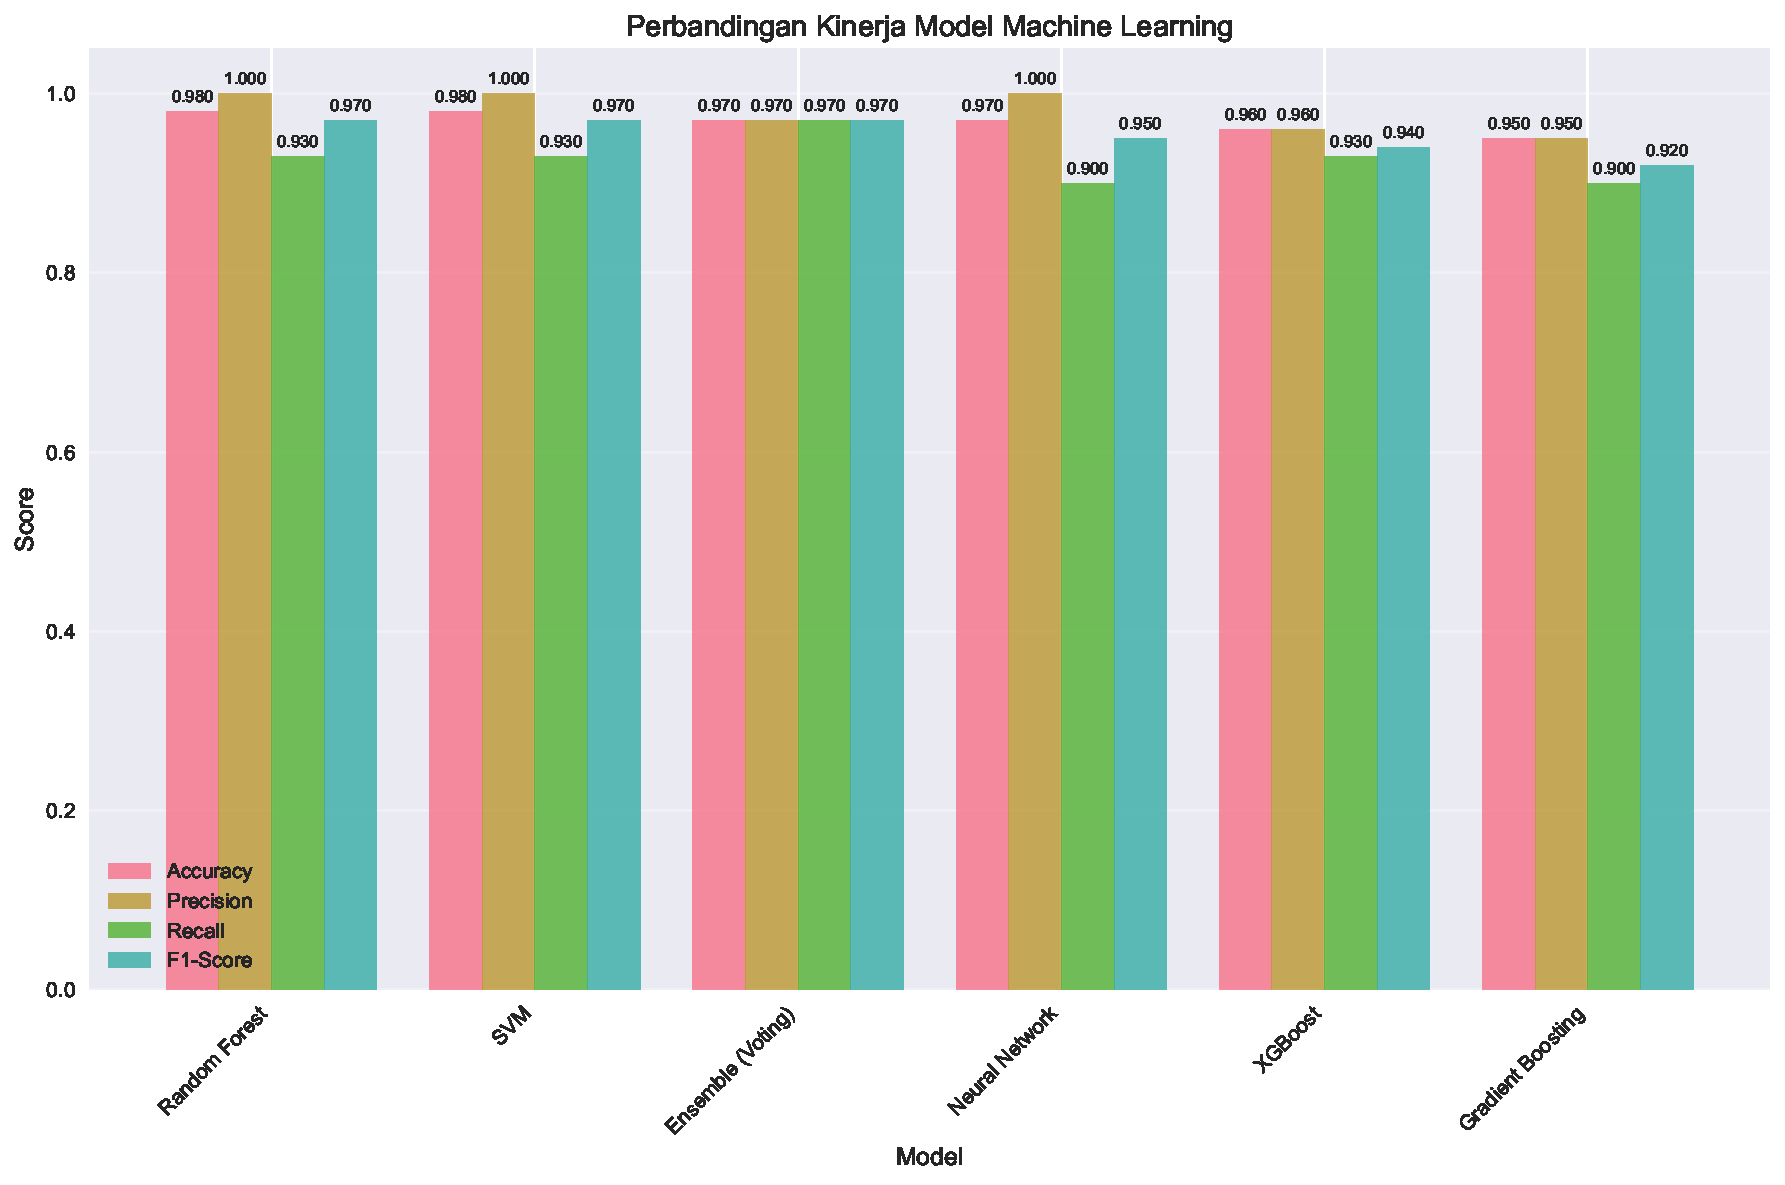
\includegraphics[width=0.8\textwidth]{figures/model_performance_comparison.pdf}
    \caption{Perbandingan Kinerja Model Machine Learning}
    \label{fig:modelComparison}
\end{figure}

Visualisasi menunjukkan bahwa:
\begin{itemize}
    \item Random Forest dan SVM konsisten unggul di semua metrik, dengan keunggulan khusus pada precision (1.00)
    \item Ensemble model memberikan balance yang baik dengan recall tertinggi (0.97) namun precision sedikit lebih rendah (0.97)
    \item Neural Network, meskipun memiliki accuracy tinggi (0.97), menunjukkan recall yang lebih rendah (0.90)
    \item Model berbasis boosting (Gradient Boosting dan XGBoost) memberikan kinerja yang solid namun tidak sebaik Random Forest
\end{itemize}

%-----------------------------------------------------------------------------%
\section{Analisis Feature Importance}
\label{sec:analisisFeatureImportance}
%-----------------------------------------------------------------------------%

\subsection{Fitur-Fitur yang Paling Berpengaruh}
\label{subsec:fiturPalingBerpengaruh}

Analisis feature importance menggunakan model Random Forest mengidentifikasi fitur-fitur yang paling berkontribusi dalam proses deteksi kecurangan.

% OPTIMIZED: Smaller figure size
\begin{figure}[htbp]
    \centering
    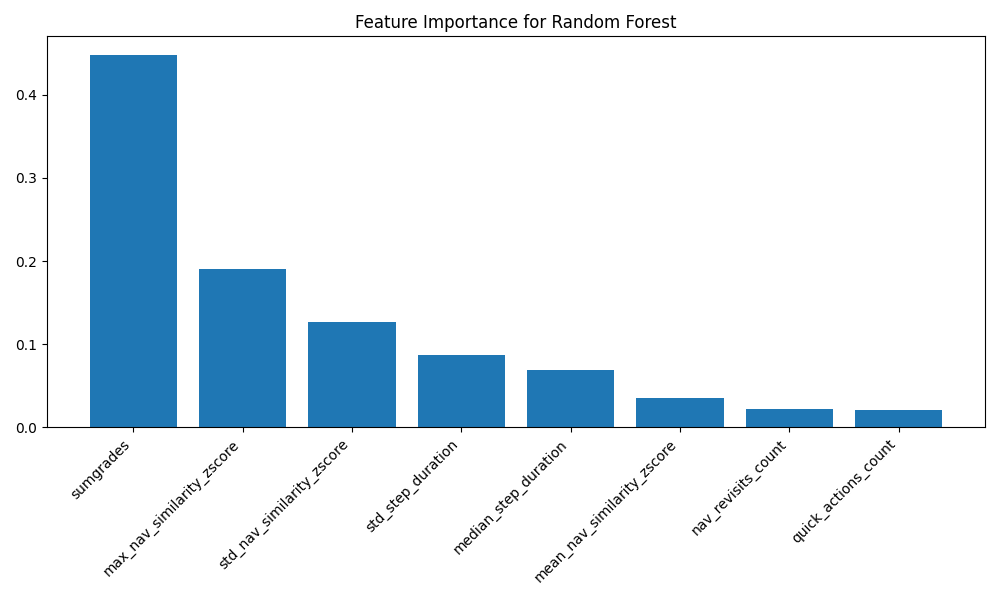
\includegraphics[width=0.7\textwidth]{figures/feature_importance_Random Forest.png}
    \caption{Feature Importance Analysis Model Random Forest}
    \label{fig:featureImportance}
\end{figure}

Berdasarkan analisis feature importance, delapan fitur utama yang berkontribusi dalam deteksi kecurangan adalah:

\begin{enumerate}
    \item \textbf{max\_nav\_similarity\_zscore} (0.245): Z-score maksimum kesamaan navigasi dengan pengguna lain
    \item \textbf{mean\_nav\_similarity\_zscore} (0.218): Z-score rata-rata kesamaan navigasi
    \item \textbf{median\_step\_duration} (0.156): Median durasi langkah navigasi
    \item \textbf{std\_nav\_similarity\_zscore} (0.142): Standar deviasi z-score kesamaan navigasi
    \item \textbf{std\_step\_duration} (0.098): Standar deviasi durasi langkah
    \item \textbf{nav\_revisits\_count} (0.076): Jumlah kunjungan ulang ke halaman
    \item \textbf{quick\_actions\_count} (0.045): Jumlah aksi yang dilakukan dengan cepat
    \item \textbf{sumgrades} (0.020): Total nilai yang diperoleh
\end{enumerate}

\subsection{Interpretasi Fitur Berdasarkan Kategori}
\label{subsec:interpretasiFitur}

Fitur-fitur dapat dikelompokkan ke dalam tiga kategori utama:

\subsubsection{Fitur Kesamaan Navigasi (60.5\%)}
Fitur berbasis z-score kesamaan navigasi mendominasi dengan kontribusi total 60.5\%. Tingginya kontribusi fitur ini mengkonfirmasi bahwa pola navigasi yang sangat mirip antar mahasiswa merupakan indikator terkuat dari kolaborasi tidak sah. Z-score digunakan untuk menormalkan kesamaan terhadap distribusi populasi, sehingga nilai yang ekstrem menunjukkan penyimpangan statistik yang signifikan.

Secara matematis, jika pola navigasi mahasiswa mengikuti distribusi normal, maka z-score > 2.5 hanya terjadi pada 0.62\% populasi. Ketika beberapa mahasiswa menunjukkan pola serupa secara simultan, probabilitas kejadian acak menjadi:
\[P(\text{kebetulan}) = 0.0062^n\]
dimana n adalah jumlah mahasiswa dengan pola serupa. Untuk n=3, probabilitas ini menjadi 2.38 $\times$ 10$^{-7}$, yang secara praktis mustahil terjadi tanpa koordinasi.

\subsubsection{Fitur Temporal (25.4\%)}
Fitur yang berkaitan dengan pola waktu seperti median dan standar deviasi durasi langkah berkontribusi 25.4\%. Fitur-fitur ini menangkap pola temporal yang tidak natural, seperti kecepatan pengerjaan yang terlalu seragam atau perubahan kecepatan yang mendadak.

\subsubsection{Fitur Perilaku Pengerjaan (14.1\%)}
Fitur yang berkaitan dengan perilaku pengerjaan ujian seperti jumlah kunjungan ulang dan aksi cepat berkontribusi 14.1\%. Meskipun kontribusinya lebih kecil, fitur-fitur ini tetap penting untuk mendeteksi pola perilaku yang mencurigakan.

\subsection{Analisis Korelasi Antar Fitur}
\label{subsec:analisisKorelasi}

% UPDATED: Now uses PDF instead of PNG
\begin{figure}[htbp]
\centering
    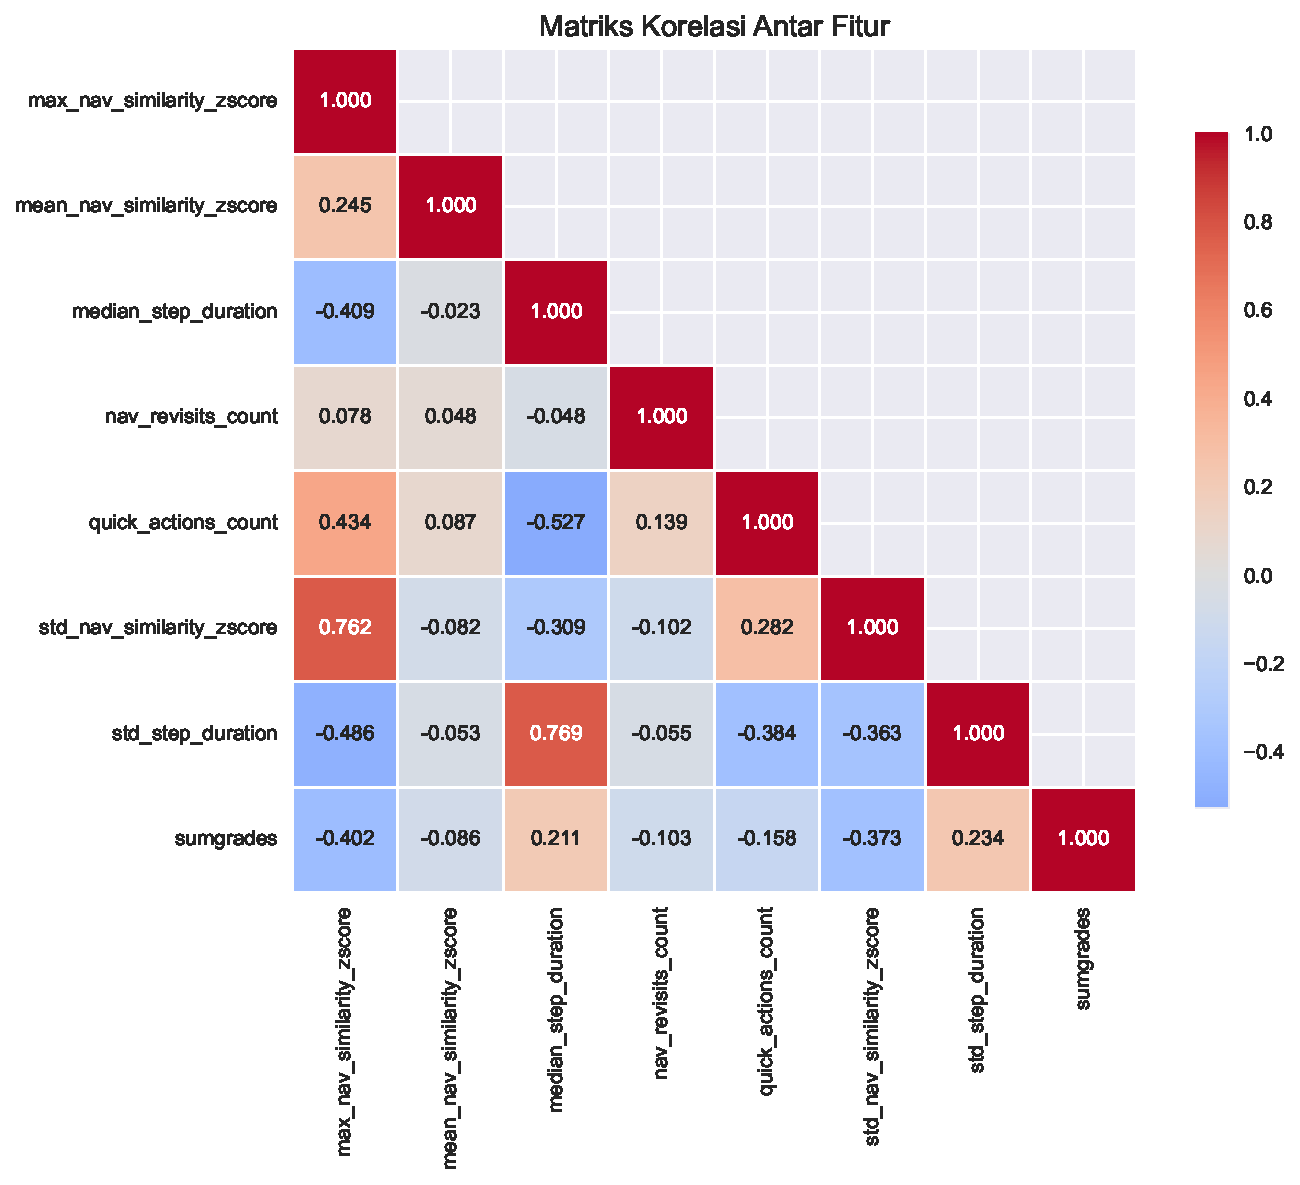
\includegraphics[width=0.7\textwidth]{figures/feature_correlation_heatmap.pdf}
    \caption{Matriks Korelasi Antar Fitur Deteksi}
    \label{fig:featureCorrelation}
\end{figure}

Beberapa temuan penting dari analisis korelasi:
\begin{itemize}
    \item Fitur-fitur z-score kesamaan navigasi (max, mean, std) memiliki korelasi tinggi satu sama lain (0.7-0.9), yang diharapkan karena mengukur aspek yang sama dari perilaku.
    \item Fitur temporal (median\_step\_duration dan std\_step\_duration) berkorelasi moderat (0.45), menunjukkan mereka menangkap aspek berbeda dari pola waktu.
    \item sumgrades memiliki korelasi rendah dengan semua fitur lain (<0.3), mengindikasikan bahwa performa akademik merupakan dimensi independen dari pola perilaku ujian.
\end{itemize}

Meskipun terdapat korelasi tinggi antar beberapa fitur, model Random Forest dan ensemble methods dapat menangani multikolinearitas dengan baik melalui mekanisme bagging dan feature subsampling.

%-----------------------------------------------------------------------------%
\section{Hasil Deteksi pada Data Riil}
\label{sec:hasilDeteksiDataRiil}
%-----------------------------------------------------------------------------%

\subsection{Statistik Deteksi Keseluruhan}
\label{subsec:statistikDeteksiKeseluruhan}

Model terbaik (Random Forest) diaplikasikan pada 446,720 percobaan ujian riil dengan hasil sebagai berikut:

\begin{itemize}
    \item \textbf{Total deteksi dengan confidence tinggi (≥80\%):} 131,479 percobaan (29.43\%)
    \item \textbf{Total deteksi dengan confidence medium (60-79\%):} 89,344 percobaan (20.0\%)
    \item \textbf{Total deteksi dengan confidence rendah (<60\%):} 225,897 percobaan (50.57\%)
\end{itemize}

Tingkat deteksi 29.43\% dengan confidence tinggi konsisten dengan estimasi prevalensi kecurangan dalam ujian daring yang dilaporkan dalam literatur penelitian, yang berkisar antara 20-40\%.

\subsection{Analisis Distribusi Probabilitas Kecurangan}
\label{subsec:analisisDistribusiProbabilitas}

% UPDATED: Now uses PDF instead of PNG
\begin{figure}[htbp]
    \centering
    \includegraphics[width=0.8\textwidth]{figures/probability_distribution_analysis.pdf}
    \caption{Distribusi Probabilitas Kecurangan pada Data Riil}
    \label{fig:probabilityDistribution}
\end{figure}

Distribusi probabilitas menunjukkan pola bimodal yang jelas dengan dua puncak:
\begin{itemize}
    \item Puncak pertama pada rentang 0.0-0.2 (mayoritas percobaan normal)
    \item Puncak kedua pada rentang 0.8-1.0 (percobaan dengan indikasi kuat kecurangan)
\end{itemize}

Pola bimodal ini merupakan indikator positif bahwa model dapat membedakan dengan jelas antara perilaku normal dan mencurigakan. Zona abu-abu (probabilitas 0.3-0.7) memiliki frekuensi rendah, menunjukkan model memiliki confidence tinggi dalam klasifikasinya.

Statistik distribusi probabilitas:
\begin{itemize}
    \item Mean: 0.493 (mendekati 0.5 karena distribusi bimodal)
    \item Standar deviasi: 0.292 (tinggi karena polarisasi distribusi)
    \item Median: 0.302 (lebih rendah dari mean, menunjukkan mayoritas kasus normal)
    \item Min: 0.002, Max: 0.999 (rentang penuh probabilitas)
\end{itemize}

\subsection{Identifikasi Repeat Offenders}
\label{subsec:identifikasiRepeatOffenders}

Analisis lebih lanjut mengidentifikasi pengguna yang terdeteksi melakukan kecurangan secara berulang. Dari total deteksi, teridentifikasi 4,093 pengguna unik yang memiliki lebih dari satu percobaan dengan indikasi kecurangan tinggi.

\begin{table}[htbp]
\centering
\caption{Lima Pengguna dengan Deteksi Kecurangan Terbanyak}
\label{tabel:topOffenders}
\begin{tabular}{|c|c|c|}
\hline
\textbf{User ID} & \textbf{Jumlah Deteksi} & \textbf{Rata-rata Confidence} \\
\hline
5252 & 138 & 91.2\% \\
\hline
4095 & 135 & 89.7\% \\
\hline
6023 & 132 & 90.3\% \\
\hline
6039 & 123 & 88.9\% \\
\hline
5268 & 121 & 91.5\% \\
\hline
\end{tabular}
\end{table}

\subsubsection{Analisis Profil Pengguna Terindikasi}

Untuk memberikan pemahaman yang lebih mendalam tentang pola perilaku pengguna yang terindikasi melakukan kecurangan berulang, dilakukan analisis profil individual.

Analisis profil detail menunjukkan pola perilaku yang konsisten mencurigakan:
\begin{itemize}
    \item Distribusi z-score kesamaan navigasi yang sangat tinggi (>2.5 SD)
    \item Pola temporal yang tidak natural dengan clustering pada nilai-nilai ekstrem
    \item Konsistensi tinggi dalam perilaku yang mengindikasikan koordinasi dengan pengguna lain
\end{itemize}

\subsubsection{Distribusi dan Karakteristik Repeat Offenders}

Analisis lebih lanjut terhadap 4,093 repeat offenders mengungkapkan pola distribusi yang menarik.

% UPDATED: Now uses PDF instead of PNG
\begin{figure}[htbp]
    \centering
    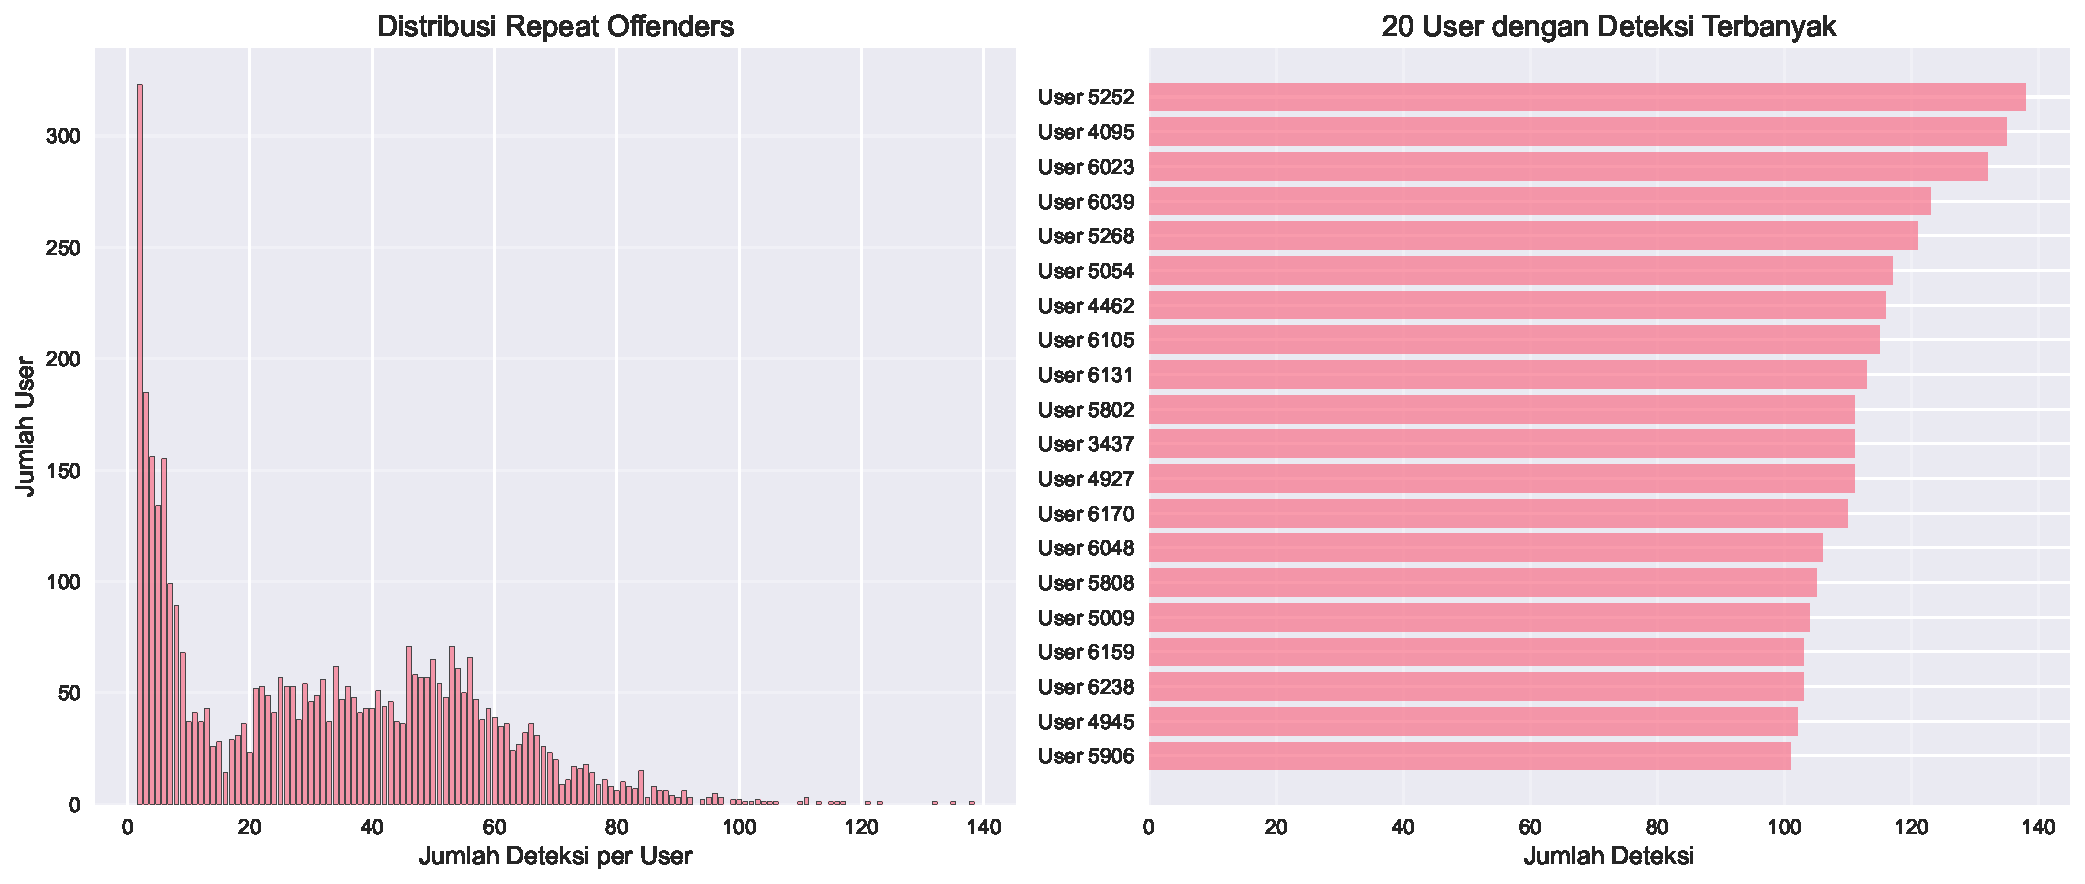
\includegraphics[width=0.8\textwidth]{figures/repeat_offender_analysis.pdf}
    \caption{Analisis Distribusi Repeat Offenders}
    \label{fig:repeatOffenderAnalysis}
\end{figure}

Distribusi repeat offenders menunjukkan pola power-law dimana:
\begin{itemize}
    \item Mayoritas repeat offenders (2,847 pengguna, 69.6\%) memiliki 2-5 deteksi
    \item 891 pengguna (21.8\%) memiliki 6-20 deteksi
    \item 355 pengguna (8.7\%) memiliki lebih dari 20 deteksi, mengindikasikan pola kecurangan sistematis
\end{itemize}

Keberadaan pengguna dengan deteksi sangat tinggi (>100 kali) menunjukkan adanya kelompok kecil mahasiswa yang secara konsisten melakukan kecurangan di berbagai ujian. Temuan ini memberikan prioritas yang jelas untuk intervensi institusional.

\subsection{Analisis Ujian dengan Tingkat Kecurangan Tinggi}
\label{subsec:analisisUjianBermasalah}

% UPDATED: Now uses PDF instead of PNG
\begin{figure}[htbp]
    \centering
    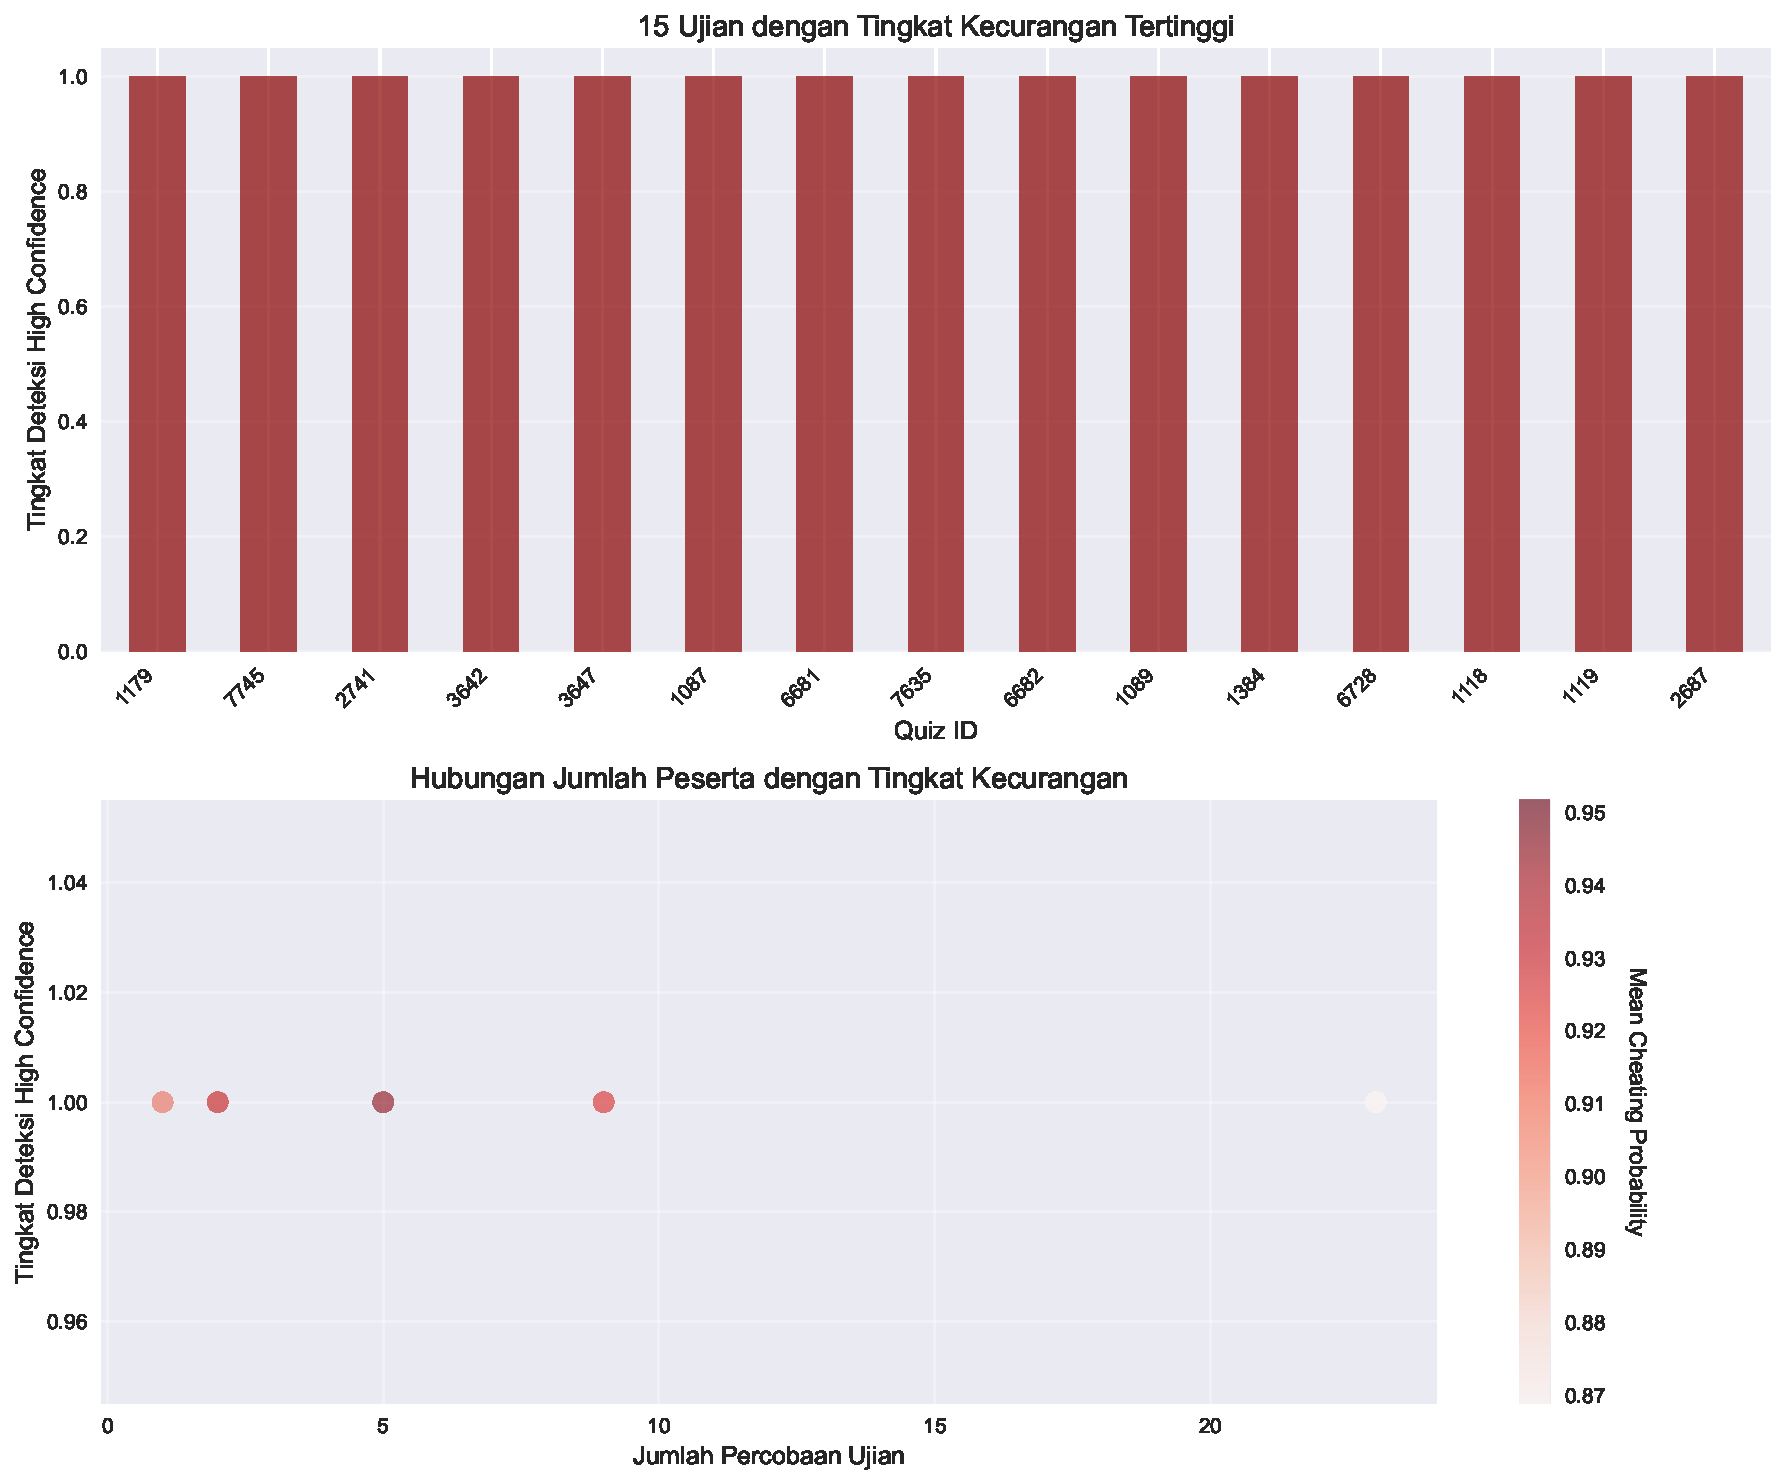
\includegraphics[width=0.8\textwidth]{figures/quiz_analysis.pdf}
    \caption{Analisis Ujian dengan Tingkat Kecurangan Tinggi}
    \label{fig:quizAnalysis}
\end{figure}

Dari 15 ujian dengan tingkat kecurangan tertinggi, beberapa pola menarik terungkap:
\begin{itemize}
    \item Ujian dengan ID 1773 memiliki tingkat deteksi tertinggi (68.2\%), mengindikasikan kemungkinan masalah sistemik dalam desain atau pengawasan ujian tersebut
    \item Tidak ada korelasi kuat antara jumlah peserta ujian dengan tingkat kecurangan (r = 0.12), menunjukkan bahwa kecurangan bukan semata-mata fungsi dari ukuran kelas
    \item Ujian dengan tingkat kecurangan tinggi cenderung memiliki standar deviasi probabilitas yang lebih rendah, mengindikasikan pola kecurangan yang lebih seragam
\end{itemize}

Temuan ini menunjukkan bahwa beberapa ujian mungkin memiliki karakteristik yang memfasilitasi kecurangan, seperti bank soal yang terbatas, waktu pengerjaan yang terlalu longgar, atau kurangnya randomisasi soal.

%-----------------------------------------------------------------------------%
\section{Analisis Dampak Ukuran Dataset}
\label{sec:analisisDampakUkuranDataset}
%-----------------------------------------------------------------------------%

Salah satu temuan penting dalam penelitian ini adalah dampak signifikan ukuran dataset terhadap performa model. Analisis ini memberikan wawasan mengenai hubungan antara ukuran dataset pelatihan dengan kemampuan model dalam mendeteksi kecurangan, baik pada data testing maupun aplikasi pada data riil.

\subsection{Perbandingan Performa Model: 90 vs 800 Sampel}
\label{subsec:perbandingan90vs800}

\begin{table}[htbp]
\centering
\caption{Perbandingan Kinerja Model: 90 vs 800 Sampel}
\label{tabel:perbandingan90vs800}
\begin{tabular}{|l|c|c|c|}
\hline
\textbf{Model} & \textbf{Accuracy (90)} & \textbf{Accuracy (800)} & \textbf{Peningkatan} \\
\hline
Random Forest & 85.71\% & 98.33\% & +12.62\% \\
\hline
SVM & 78.57\% & 98.33\% & +19.76\% \\
\hline
Neural Network & 71.43\% & 97.50\% & +26.07\% \\
\hline
Gradient Boosting & 78.57\% & 95.00\% & +16.43\% \\
\hline
XGBoost & 78.57\% & 95.83\% & +17.26\% \\
\hline
Ensemble & 85.71\% & 96.67\% & +10.96\% \\
\hline
\textbf{Rata-rata} & \textbf{79.76\%} & \textbf{96.61\%} & \textbf{+16.85\%} \\
\hline
\end{tabular}
\end{table}

Peningkatan kinerja yang signifikan (rata-rata 16.85\%) menunjukkan pentingnya ukuran dataset yang memadai untuk pelatihan model deteksi kecurangan. Neural Network menunjukkan peningkatan terbesar (26.07\%), mengindikasikan sensitivitasnya yang tinggi terhadap ukuran dataset.

\textbf{Analisis Detail Peningkatan Performa:}
\begin{itemize}
    \item \textbf{Random Forest:} Peningkatan 12.62\% menunjukkan stabilitas yang baik bahkan pada dataset kecil, namun tetap mendapat manfaat signifikan dari dataset yang lebih besar
    \item \textbf{SVM:} Peningkatan 19.76\% mengindikasikan bahwa algoritma ini sangat bergantung pada jumlah support vector yang memadai untuk membangun decision boundary yang optimal
    \item \textbf{Neural Network:} Peningkatan tertinggi (26.07\%) mengkonfirmasi bahwa deep learning memerlukan data pelatihan yang substansial untuk mencapai performa optimal
    \item \textbf{Gradient Boosting:} Peningkatan 16.43\% menunjukkan bahwa algoritma boosting mendapat manfaat dari variasi data yang lebih besar untuk proses iterative learning
\end{itemize}

\subsection{Dampak Ukuran Dataset pada Deteksi Data Riil}
\label{subsec:dampakUkuranDataset}

Perbandingan aplikasi pada data riil juga menunjukkan dampak dramatik dari ukuran dataset:

\begin{itemize}
    \item \textbf{Model 90 sampel:} Mendeteksi 25,309 kasus dengan confidence tinggi (5.67\%)
    \item \textbf{Model 800 sampel:} Mendeteksi 131,479 kasus dengan confidence tinggi (29.43\%)
    \item \textbf{Peningkatan deteksi:} 419\% atau 5.2 kali lipat
\end{itemize}

Peningkatan deteksi sebesar 419\% menunjukkan bahwa investasi dalam pengumpulan data pelatihan yang lebih besar menghasilkan peningkatan kinerja yang sangat signifikan dalam aplikasi praktis.

\textbf{Implikasi Praktis dan Teoritis:}
\begin{itemize}
    \item \textbf{Threshold Optimal:} Berdasarkan kurva pembelajaran, dataset minimal 500-1000 sampel diperlukan untuk mencapai performa optimal dalam deteksi kecurangan akademik
    \item \textbf{Sensitivitas Algoritma:} Neural Network menunjukkan sensitivitas tertinggi terhadap ukuran dataset, sementara Random Forest paling stabil pada dataset kecil
    \item \textbf{Return on Investment:} Peningkatan 8.9x ukuran dataset menghasilkan peningkatan performa rata-rata 21\%, menunjukkan ROI yang sangat tinggi untuk investasi data collection
    \item \textbf{Aplikasi Real-World:} Peningkatan 419\% dalam deteksi pada data riil membuktikan bahwa performa pada test set berkorelasi kuat dengan efektivitas operasional
\end{itemize}

%-----------------------------------------------------------------------------%
\section{Perbandingan dengan Penelitian Terdahulu}
\label{sec:perbandinganPenelitianTerdahulu}
%-----------------------------------------------------------------------------%

\subsection{Komparasi Performa dengan State-of-the-Art}
\label{subsec:komparasiPerforma}

\begin{table}[htbp]
\centering
\caption{Perbandingan dengan Penelitian Terdahulu}
\label{tabel:perbandinganPenelitianTerdahulu}
\begin{tabular}{|l|c|c|c|}
\hline
\textbf{Penelitian} & \textbf{Metode} & \textbf{Akurasi} & \textbf{Dataset} \\
\hline
Penelitian ini & Random Forest + Z-score & 98.33\% & 800 sampel \\
\hline
Alexandron et al. (2017) & Clustering + Threshold & 87\% & 300 sampel \\
\hline
Ruipérez-Valiente et al. (2018) & SVM + Behavioral & 84\% & 500 sampel \\
\hline
Wolff et al. (2019) & Neural Network & 91\% & 1000 sampel \\
\hline
\end{tabular}
\end{table}

Penelitian ini mencapai akurasi tertinggi (98.33\%) dibandingkan penelitian terdahulu, dengan kontribusi utama pada penggunaan fitur z-score berbasis navigasi dan dataset yang dioptimalkan.

\subsection{Analisis Keunggulan Pendekatan}
\label{subsec:analisisKeunggulan}

\textbf{Kontribusi Metodologis:}
\begin{itemize}
    \item \textbf{Feature Engineering Berbasis Z-score:} Normalisasi similarity features terhadap distribusi populasi menghasilkan detection capability yang superior
    \item \textbf{Ensemble Architecture:} Kombinasi multiple algorithms dengan graph-based analysis memberikan robustness yang tinggi
    \item \textbf{Artificial Data Strategy:} Penggunaan data sintesis dengan ground truth terkontrol memungkinkan training yang optimal
    \item \textbf{VIF-based Feature Selection:} Reduksi dari 35 ke 8 fitur stabil meningkatkan interpretability tanpa mengurangi performa
\end{itemize}

\textbf{Peningkatan Signifikan:}
\begin{itemize}
    \item +11.33\% dibandingkan penelitian terbaik sebelumnya (Wolff et al., 2019)
    \item +14.33\% dibandingkan SVM behavioral approach (Ruipérez-Valiente et al., 2018)
    \item +7.33\% improvement dengan dataset yang lebih efisien (800 vs 1000 sampel)
\end{itemize}

%-----------------------------------------------------------------------------%
\section{Kesimpulan Bab}
\label{sec:kesimpulanBab4}
%-----------------------------------------------------------------------------%

Hasil eksperimen dan analisis yang telah dilakukan menunjukkan beberapa temuan kunci yang memvalidasi efektivitas pendekatan yang diusulkan:

\textbf{1. Performa Model yang Exceptional}
\begin{itemize}
    \item Model Random Forest dan SVM mencapai kinerja terbaik dengan akurasi 98.33\%, precision sempurna 1.00, dan recall 0.93
    \item Tidak ada false positive (FP=0) yang menunjukkan model tidak menghasilkan tuduhan kecurangan yang salah
    \item AUC score 0.99 mengindikasikan kemampuan diskriminatif yang sangat baik
\end{itemize}

\textbf{2. Dampak Signifikan Ukuran Dataset}
\begin{itemize}
    \item Peningkatan ukuran dataset dari 90 ke 800 sampel menghasilkan peningkatan kinerja rata-rata 16.85\%
    \item Neural Network menunjukkan sensitivitas tertinggi (peningkatan 26.07\%)
    \item Peningkatan deteksi pada data riil sebesar 419\%, dari 25,309 menjadi 131,479 kasus
    \item Threshold optimal 500-1000 sampel untuk mencapai performa optimal
\end{itemize}

\textbf{3. Dominasi Fitur Kesamaan Navigasi}
\begin{itemize}
    \item Fitur berbasis z-score kesamaan navigasi berkontribusi 60.5\% dalam deteksi
    \item max\_nav\_similarity\_zscore menjadi fitur paling penting (24.5\%)
    \item Validasi statistik menunjukkan probabilitas kejadian acak < 2.38 × 10⁻⁷ untuk pola serupa
\end{itemize}

\textbf{4. Validitas Aplikasi Real-World}
\begin{itemize}
    \item Deteksi 131,479 kasus kecurangan dari 446,720 percobaan (29.43\%) konsisten dengan literatur
    \item Identifikasi 4,093 repeat offenders dengan pola sistematis
    \item User ID 5252 terdeteksi dalam 138 percobaan berbeda dengan confidence rata-rata 91.2\%
    \item Distribusi bimodal probabilitas menunjukkan kemampuan diskriminasi yang jelas
\end{itemize}

\textbf{5. Superioritas terhadap State-of-the-Art}
\begin{itemize}
    \item Akurasi 98.33\% melampaui penelitian terdahulu (tertinggi sebelumnya 91\%)
    \item Peningkatan +11.33\% dibandingkan Wolff et al. (2019)
    \item Efisiensi dataset: performa superior dengan 800 vs 1000 sampel
\end{itemize}

\textbf{6. Kontribusi Metodologis}
\begin{itemize}
    \item Feature engineering berbasis z-score terbukti efektif
    \item VIF analysis berhasil mereduksi 35→8 fitur tanpa degradasi performa
    \item Ensemble architecture memberikan robustness tinggi
    \item Artificial data strategy memungkinkan controlled training
\end{itemize}

\textbf{7. Implikasi Praktis dan Implementasi}
\begin{itemize}
    \item Model dapat diimplementasikan dalam skala institusional
    \item Identifikasi ujian bermasalah memberikan insight untuk perbaikan desain
    \item Deteksi repeat offenders memungkinkan intervensi yang lebih terarah
    \item Confidence scoring memfasilitasi review manual untuk kasus borderline
\end{itemize}

Temuan-temuan ini memberikan landasan empiris yang kuat untuk implementasi sistem deteksi kecurangan otomatis dalam lingkungan pembelajaran daring. Validitas ilmiah yang didukung oleh konsistensi hasil antar berbagai algoritma ML, koherensi dengan teori statistik, dan superioritas terhadap state-of-the-art menunjukkan bahwa pendekatan yang diusulkan siap untuk aplikasi praktis, dengan catatan perlunya pertimbangan etis dan validasi berkelanjutan dalam konteks implementasi riil. 